\documentclass[11pt,a4paper]{article}

\usepackage[T1]{fontenc}
\usepackage[utf8]{inputenc}
\usepackage[french]{babel}
\usepackage[a4paper,margin=2.2cm]{geometry}

\usepackage{booktabs}
\usepackage{longtable}
\usepackage{array}
\usepackage[table]{xcolor}
\usepackage{graphicx}
\usepackage{hyperref}

\hypersetup{
  colorlinks=true,
  linkcolor=black,
  urlcolor=blue
}

\definecolor{softgray}{RGB}{245,245,245}

\newcolumntype{L}[1]{>{\raggedright\arraybackslash}p{#1}}
\newcolumntype{R}[1]{>{\raggedleft\arraybackslash}p{#1}}

\newcommand{\EUR}[1]{#1~\texteuro}

\title{\textbf{Budget daté du 25/03/2024}}
\author{Telecom Espoir}
\date{}

\begin{document}
\maketitle

\section*{Résumé}
\begin{itemize}
  \item Total entrées : \EUR{20483.88}
  \item Total sorties : \EUR{16949.47}
  \item Bilan net : \EUR{3534.41}
\end{itemize}

\bigskip

\section*{Synthèse globale par activité}
\rowcolors{2}{softgray}{white}
\begin{tabular}{L{6.2cm} R{3.2cm} R{3.2cm} R{3.2cm}}
\toprule
\textbf{Activité} & \textbf{Entrées} & \textbf{Sorties} & \textbf{Bilan} \\
\midrule
administratif & \EUR{0.00} & \EUR{146.79} & \EUR{-146.79} \\
autre & \EUR{1550.00} & \EUR{0.00} & \EUR{1550.00} \\
epicerie\_solidaire & \EUR{4900.00} & \EUR{1183.25} & \EUR{3716.75} \\
evenement\_telecom & \EUR{147.00} & \EUR{0.00} & \EUR{147.00} \\
evenement\_telespoir & \EUR{7549.73} & \EUR{6028.35} & \EUR{1521.38} \\
maraude & \EUR{0.00} & \EUR{276.82} & \EUR{-276.82} \\
mission\_humanitaire & \EUR{6337.15} & \EUR{9314.26} & \EUR{-2977.11} \\

\bottomrule
\end{tabular}
\rowcolors{2}{}{}

\bigskip

\begin{center}
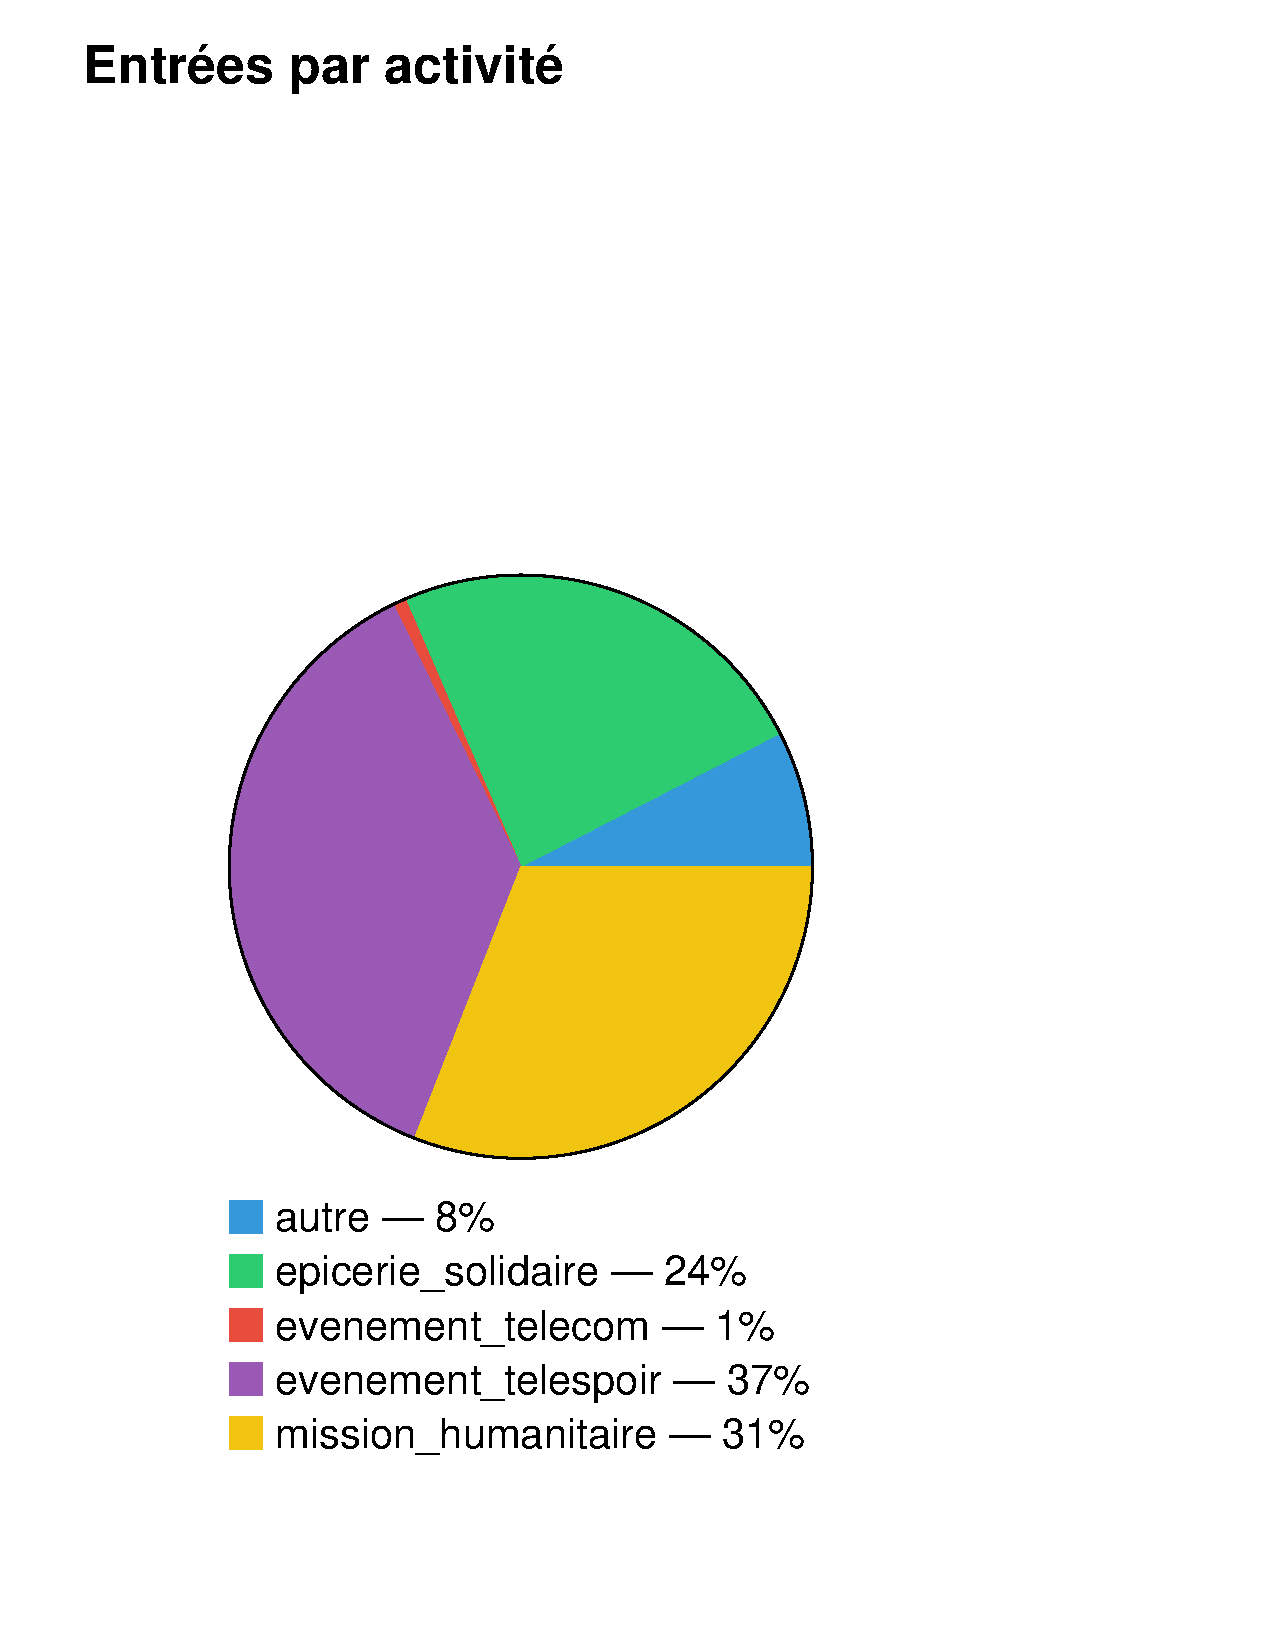
\includegraphics[width=0.46\textwidth]{charts/global_income_by_activity.pdf}
\hfill
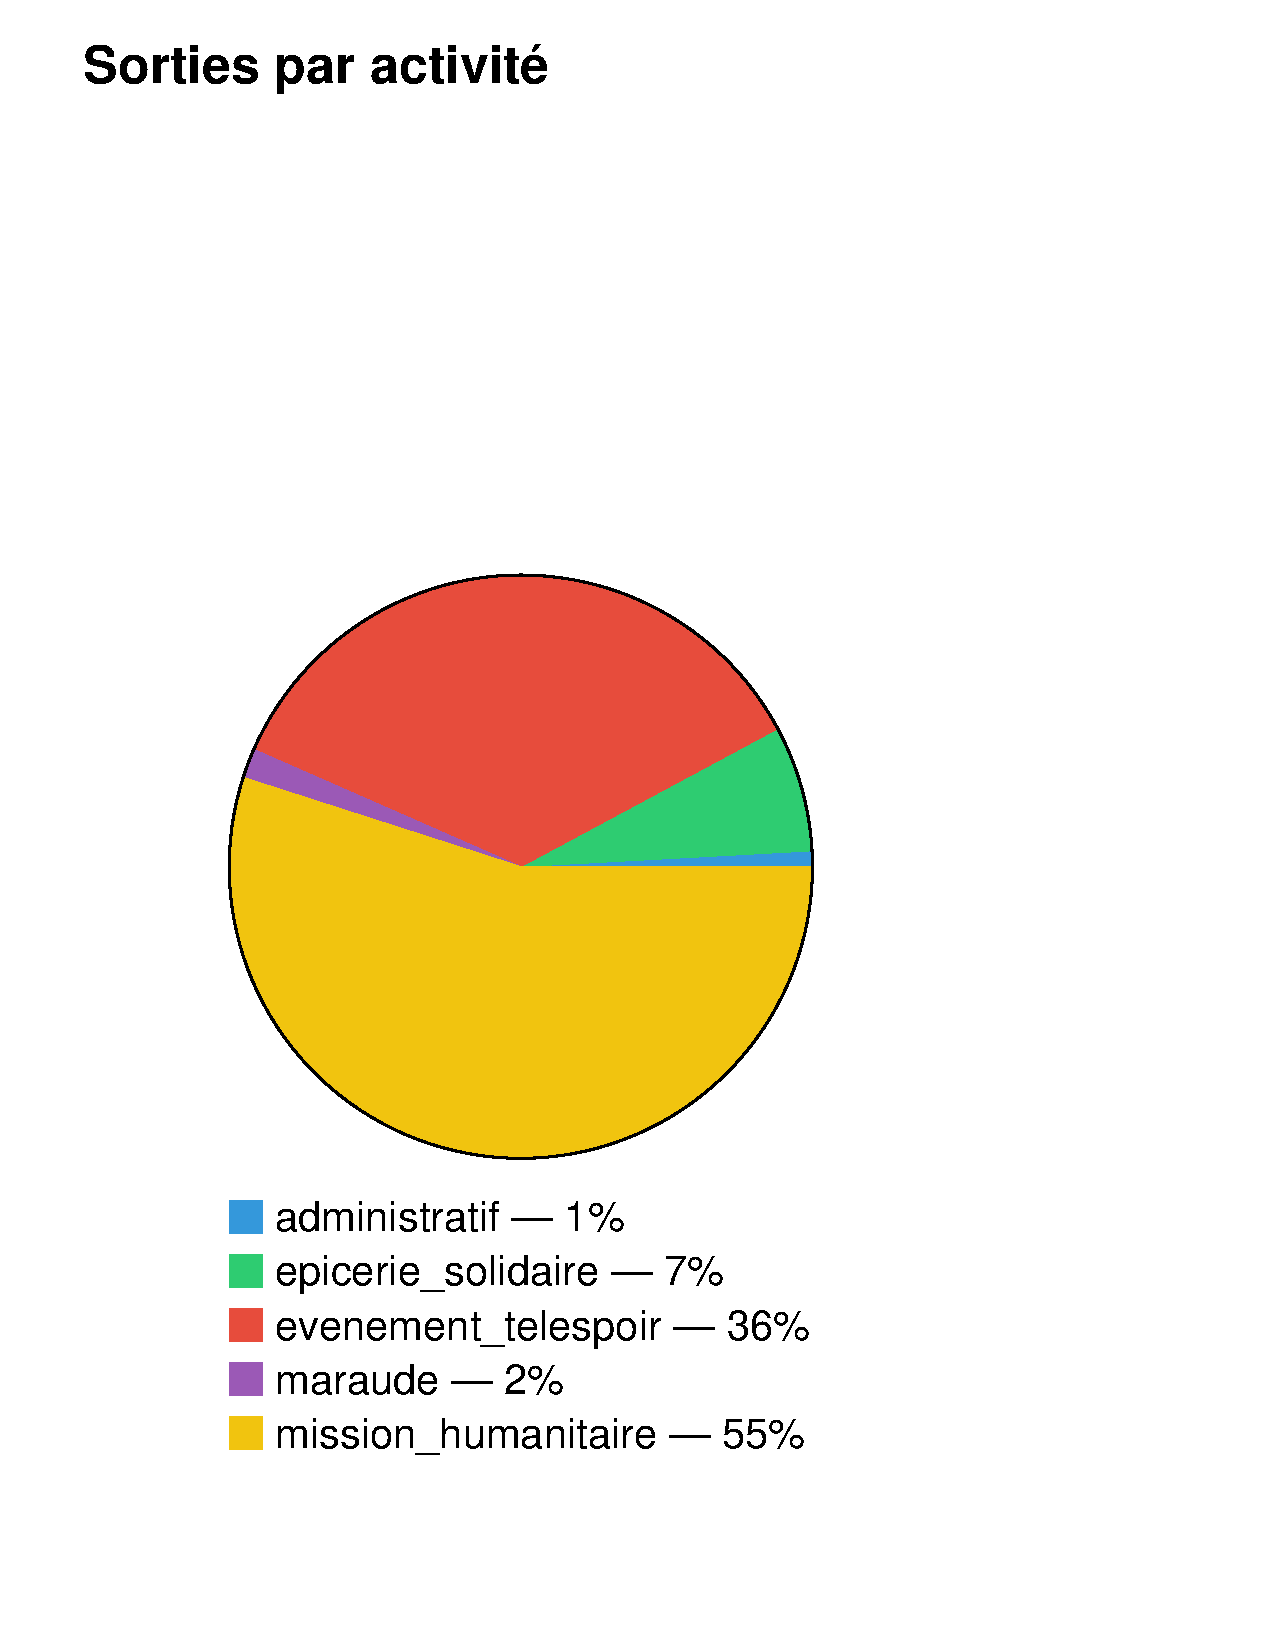
\includegraphics[width=0.46\textwidth]{charts/global_expense_by_activity.pdf}
\end{center}

\newpage

\section*{administratif}

\subsection*{Tableau des écritures}
\rowcolors{2}{softgray}{white}
\begin{longtable}{L{2.7cm} L{8.2cm} R{3.0cm}}
\toprule
\textbf{Date} & \textbf{Description} & \textbf{Montant} \\
\midrule
01/07/2023 & Frais de gestion & \EUR{-25.07} \\
15/05/2023 & Domaine internet & \EUR{-8.39} \\
15/05/2023 & Domaine internet & \EUR{-5.99} \\
17/04/2023 & assurance annuelle & \EUR{-107.34} \\

\bottomrule
\end{longtable}
\rowcolors{2}{}{}

\subsection*{Répartition}
\begin{center}

\includegraphics[width=0.46\textwidth]{charts/administratif_income.pdf}
\hfill
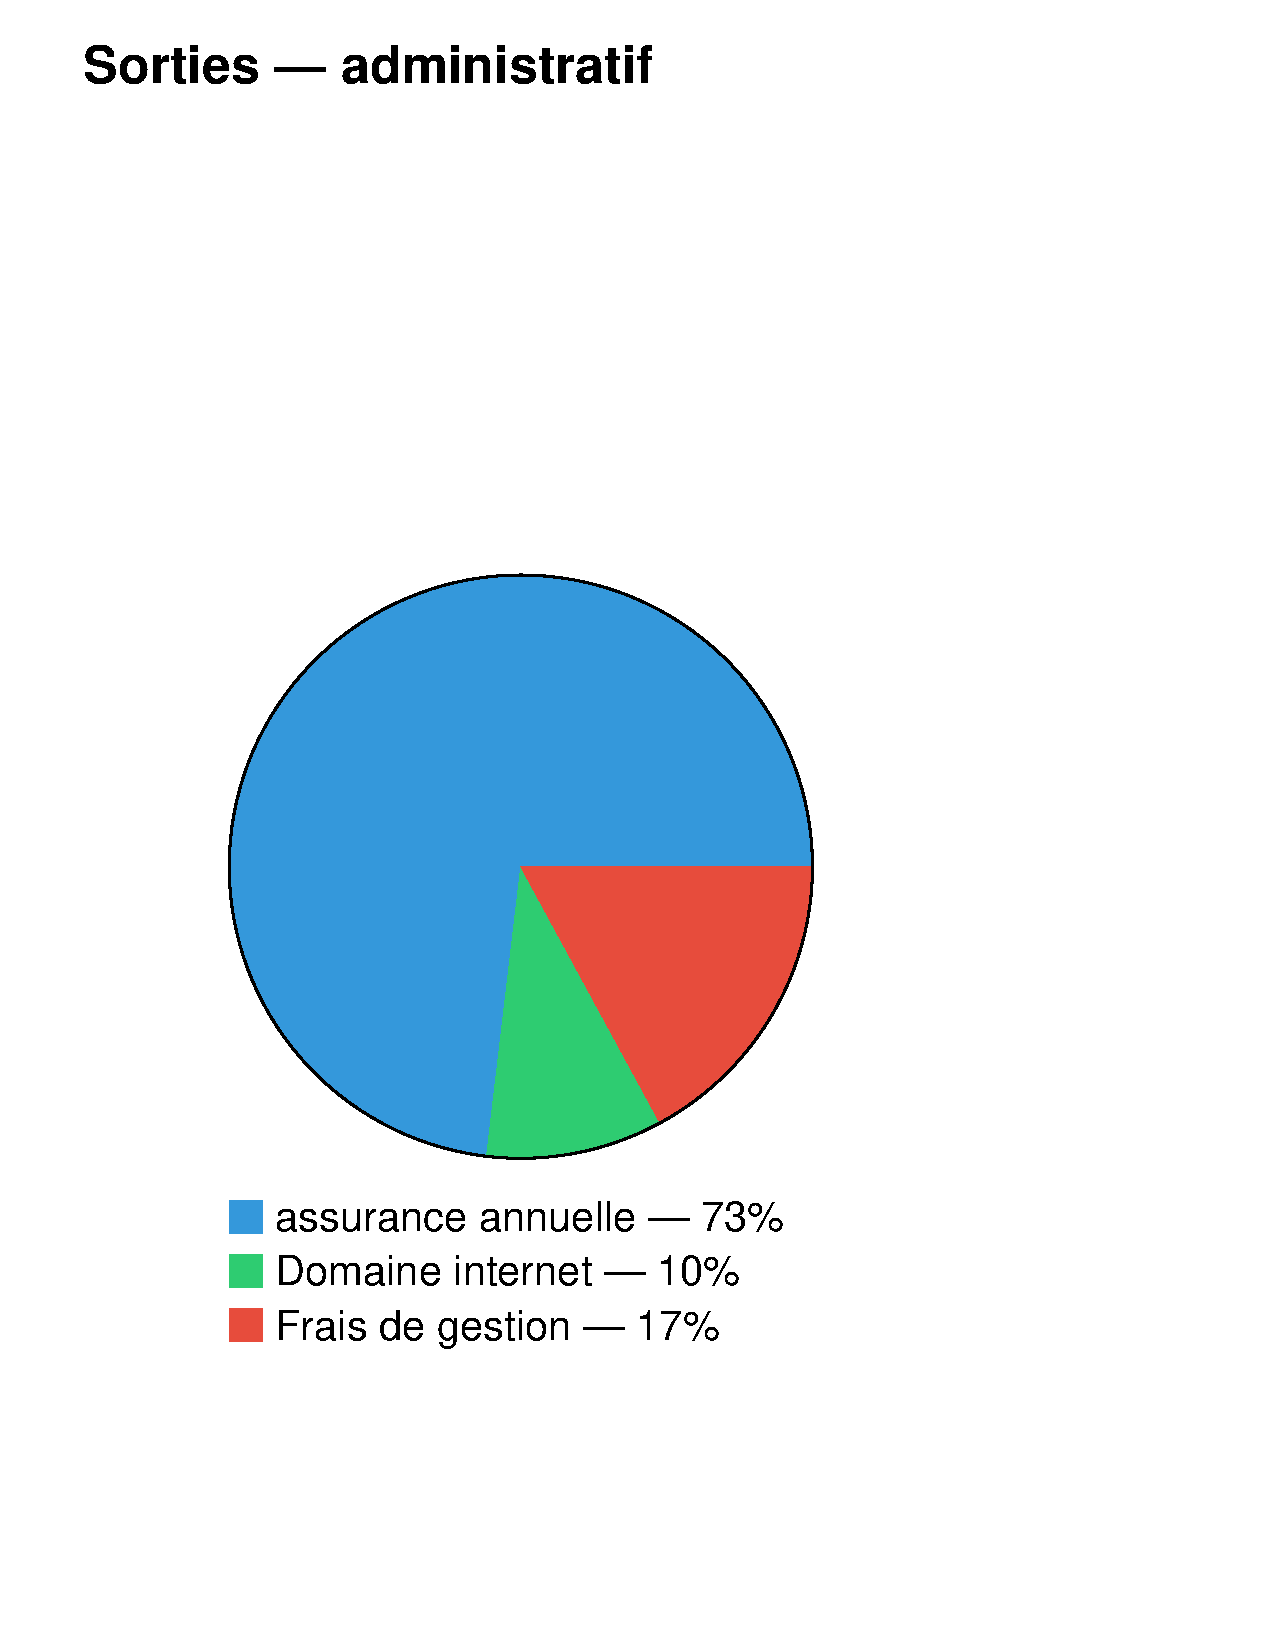
\includegraphics[width=0.46\textwidth]{charts/administratif_expense.pdf}
\end{center}

\bigskip
\textbf{Bilan activité :} \EUR{-146.79}

\newpage
\section*{autre}

\subsection*{Tableau des écritures}
\rowcolors{2}{softgray}{white}
\begin{longtable}{L{2.7cm} L{8.2cm} R{3.0cm}}
\toprule
\textbf{Date} & \textbf{Description} & \textbf{Montant} \\
\midrule
23/05/2023 & renouvellement partenariat ActiViam & \EUR{1000.00} \\
24/02/2024 & Hello/Asso & \EUR{550.00} \\

\bottomrule
\end{longtable}
\rowcolors{2}{}{}

\subsection*{Répartition}
\begin{center}
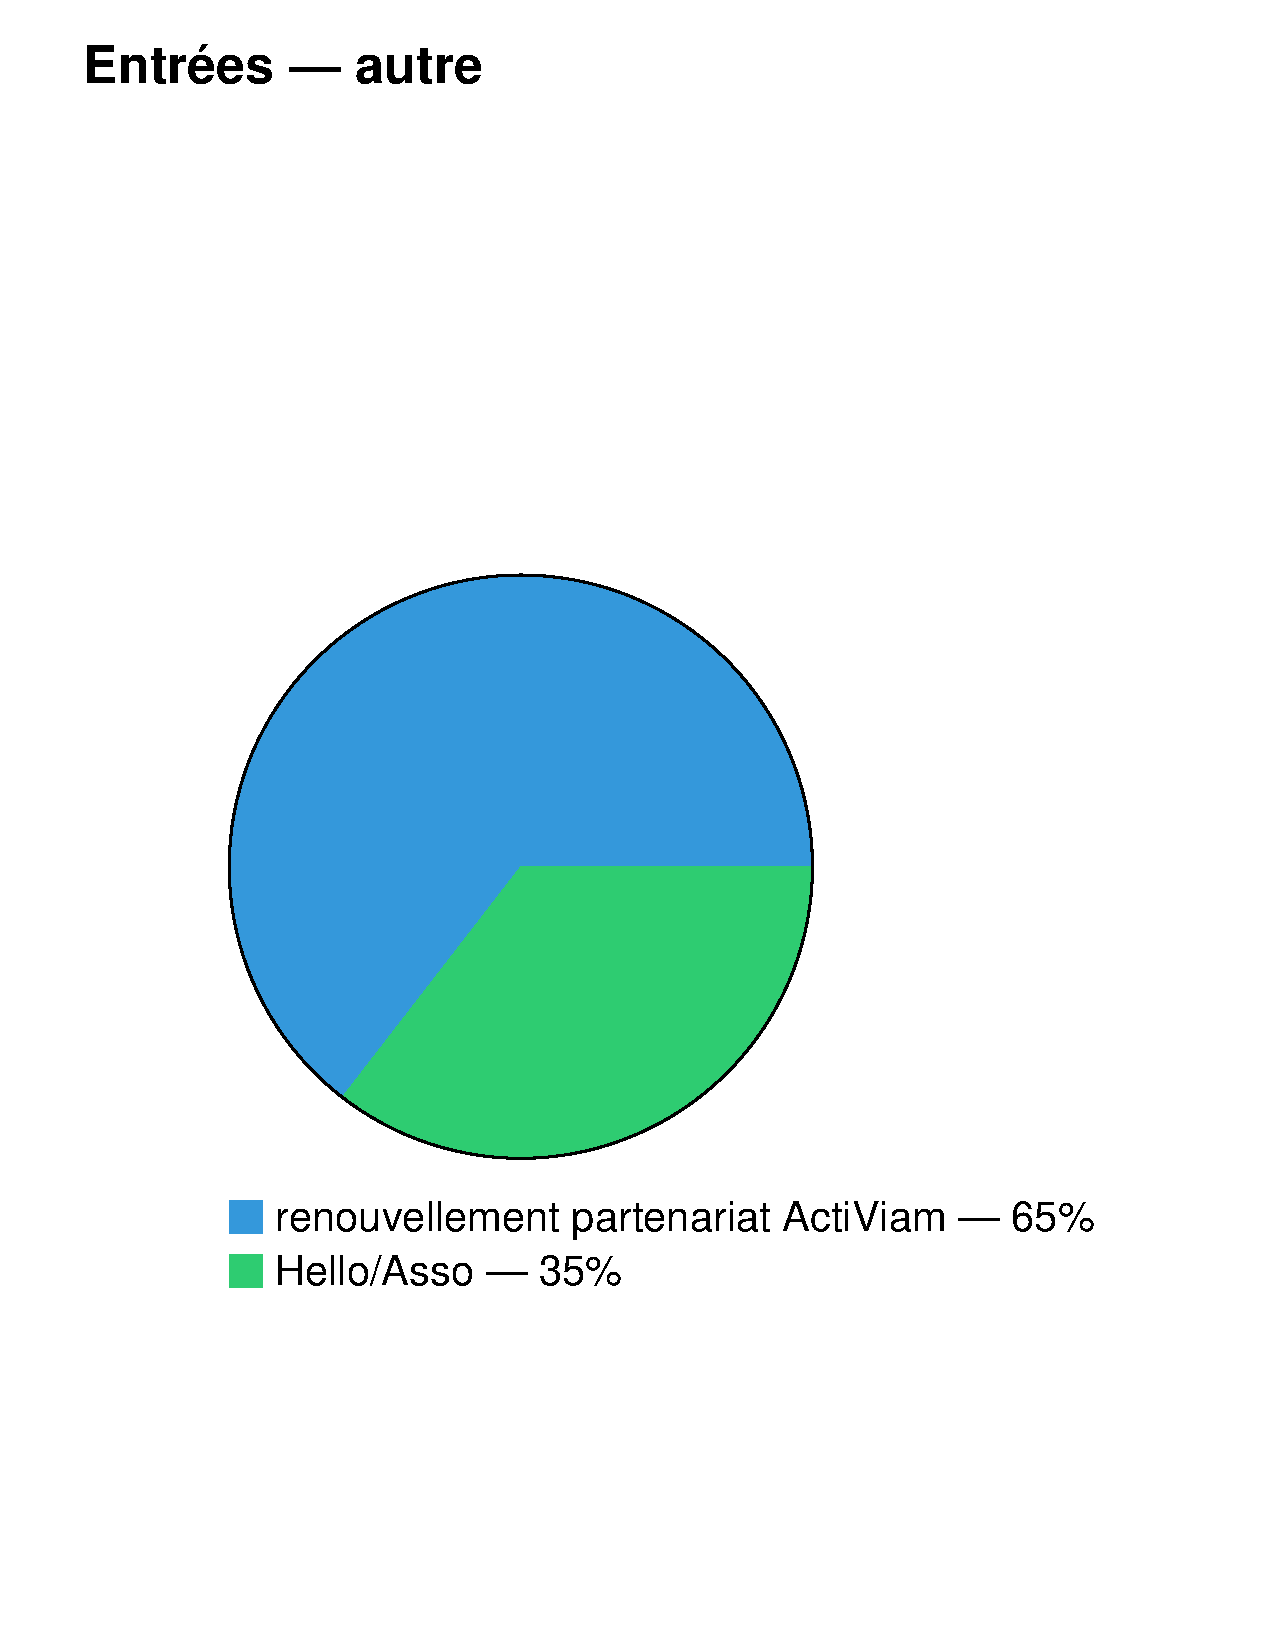
\includegraphics[width=0.46\textwidth]{charts/autre_income.pdf}
\hfill

\includegraphics[width=0.46\textwidth]{charts/autre_expense.pdf}
\end{center}

\bigskip
\textbf{Bilan activité :} \EUR{1550.00}

\newpage
\section*{epicerie\_solidaire}

\subsection*{Tableau des écritures}
\rowcolors{2}{softgray}{white}
\begin{longtable}{L{2.7cm} L{8.2cm} R{3.0cm}}
\toprule
\textbf{Date} & \textbf{Description} & \textbf{Montant} \\
\midrule
02/01/2024 & Subvention Forum ES & \EUR{1900.00} \\
03/12/2023 & 6e courses ES & \EUR{-78.13} \\
04/12/2023 & 6e courses ES & \EUR{-23.33} \\
15/05/2023 & 3e courses ES & \EUR{-37.92} \\
15/05/2023 & 3e courses ES & \EUR{-107.04} \\
19/02/2024 & 8e courses ES & \EUR{-276.14} \\
21/06/2023 & courses ES 5 & \EUR{-101.24} \\
24/03/2023 & Premières courses ES & \EUR{-175.97} \\
24/03/2023 & Premières courses ES & \EUR{-54.40} \\
24/04/2023 & 2e courses ES & \EUR{-35.69} \\
24/04/2023 & 2e courses ES & \EUR{-156.27} \\
30/05/2023 & 4e courses ES & \EUR{-42.37} \\
30/05/2023 & 4e courses ES & \EUR{-94.75} \\
30/10/2023 & Convention pour l'ES & \EUR{3000.00} \\

\bottomrule
\end{longtable}
\rowcolors{2}{}{}

\subsection*{Répartition}
\begin{center}
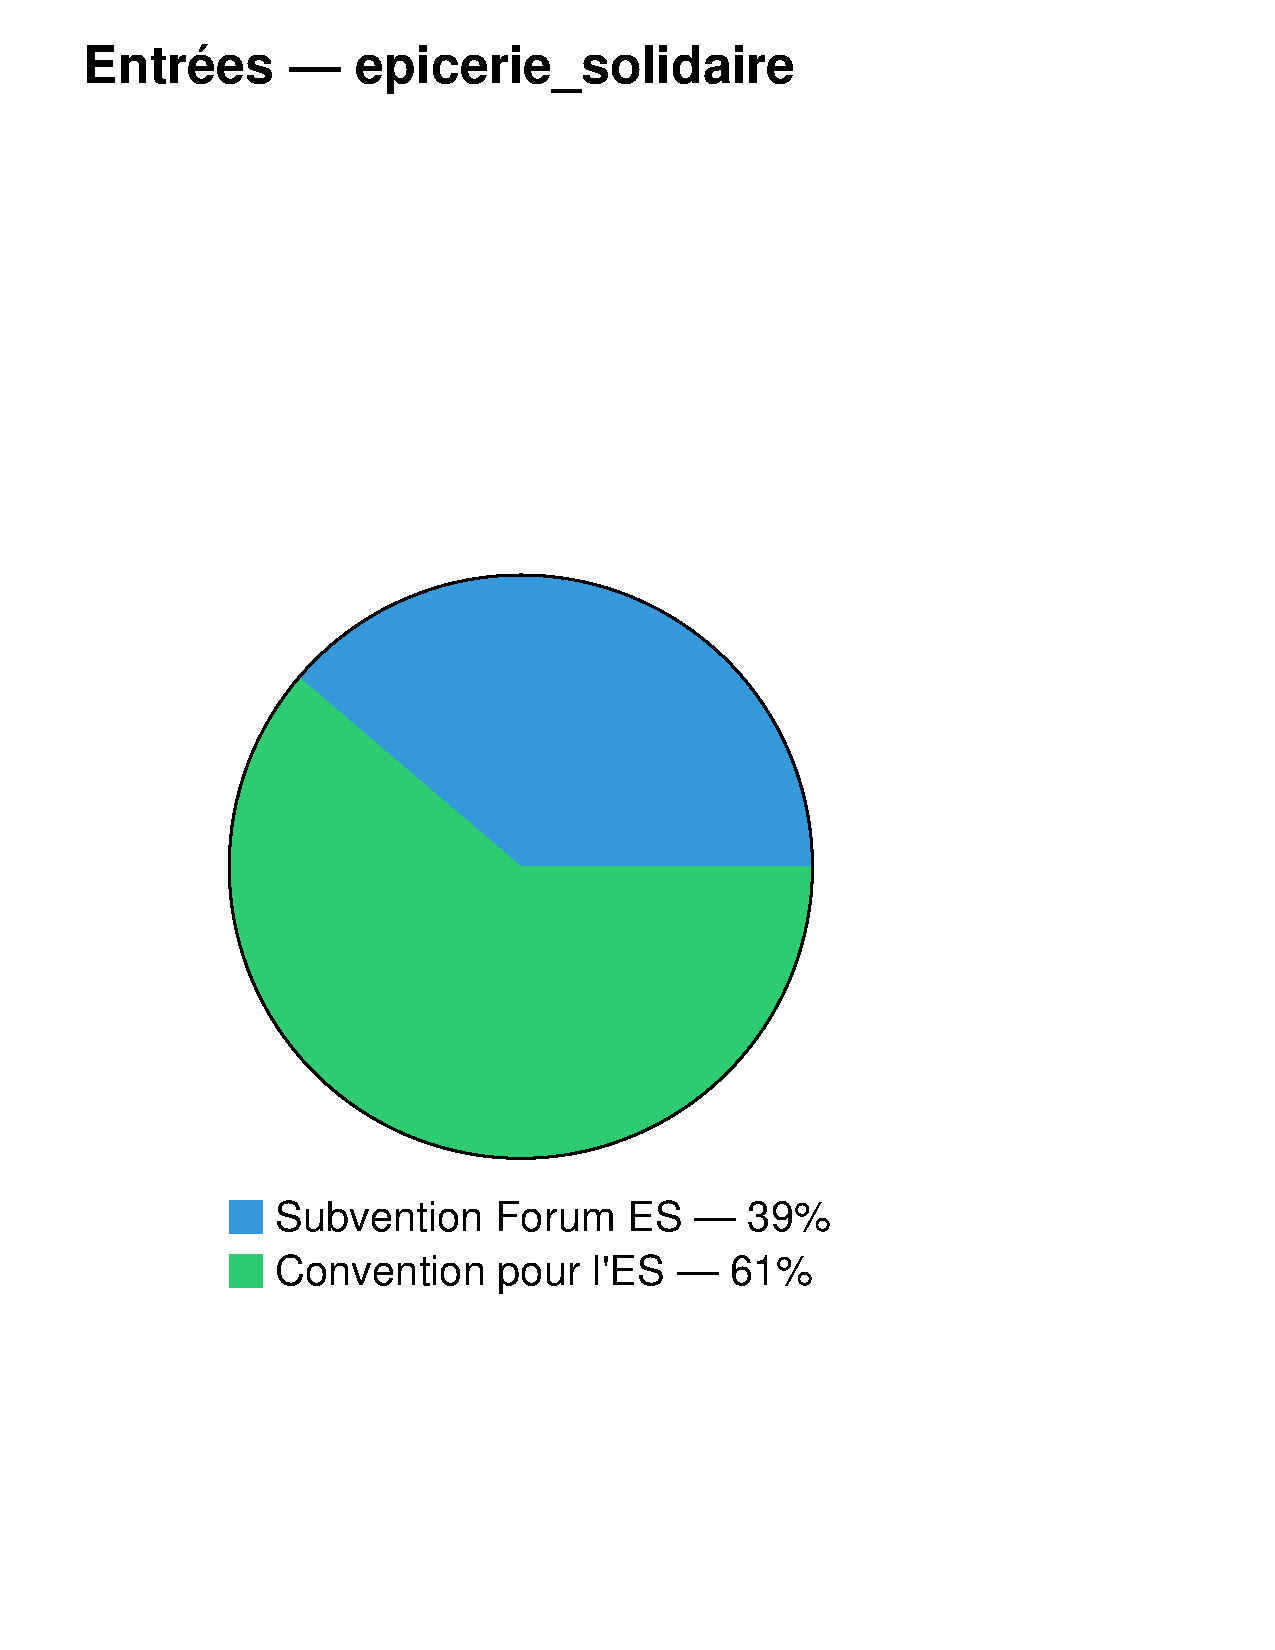
\includegraphics[width=0.46\textwidth]{charts/epicerie_solidaire_income.pdf}
\hfill
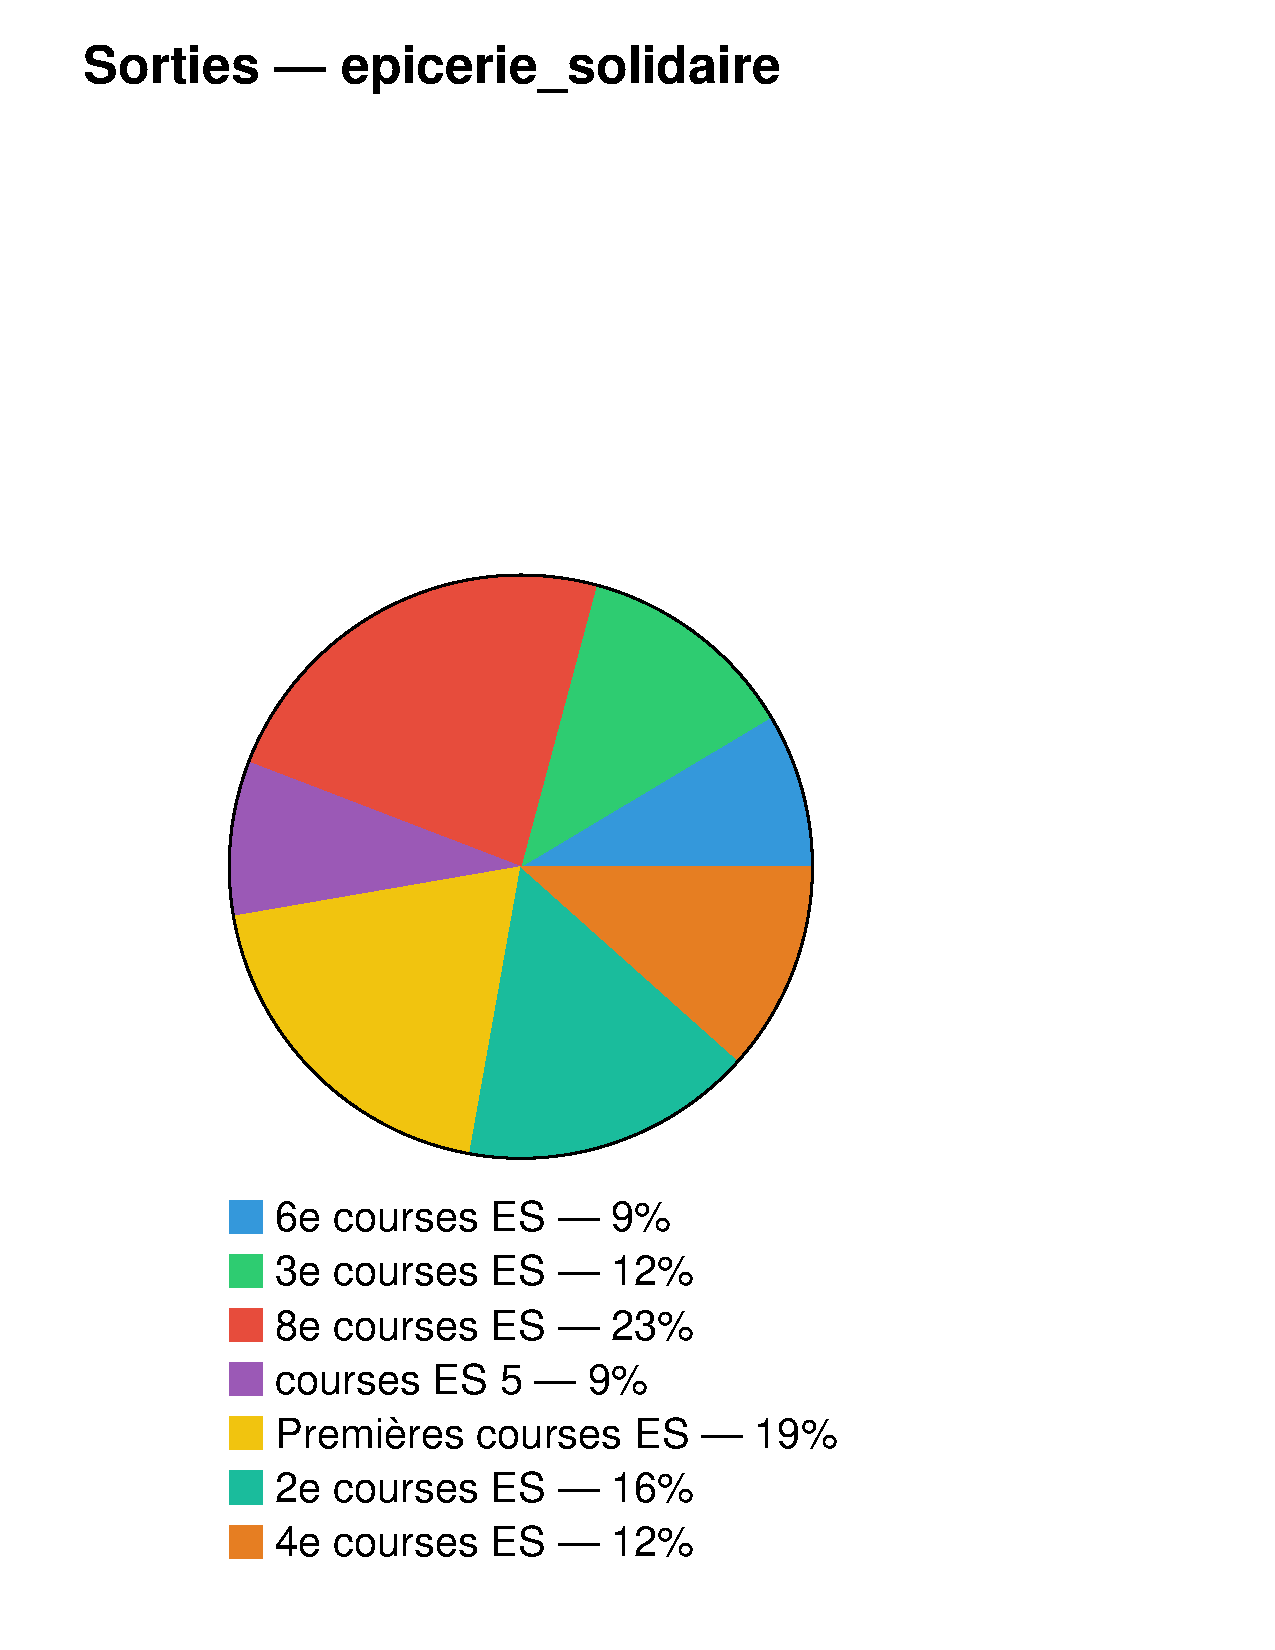
\includegraphics[width=0.46\textwidth]{charts/epicerie_solidaire_expense.pdf}
\end{center}

\bigskip
\textbf{Bilan activité :} \EUR{3716.75}

\newpage
\section*{evenement\_telecom}

\subsection*{Tableau des écritures}
\rowcolors{2}{softgray}{white}
\begin{longtable}{L{2.7cm} L{8.2cm} R{3.0cm}}
\toprule
\textbf{Date} & \textbf{Description} & \textbf{Montant} \\
\midrule
 & Recettes friperie & \EUR{147.00} \\

\bottomrule
\end{longtable}
\rowcolors{2}{}{}

\subsection*{Répartition}
\begin{center}
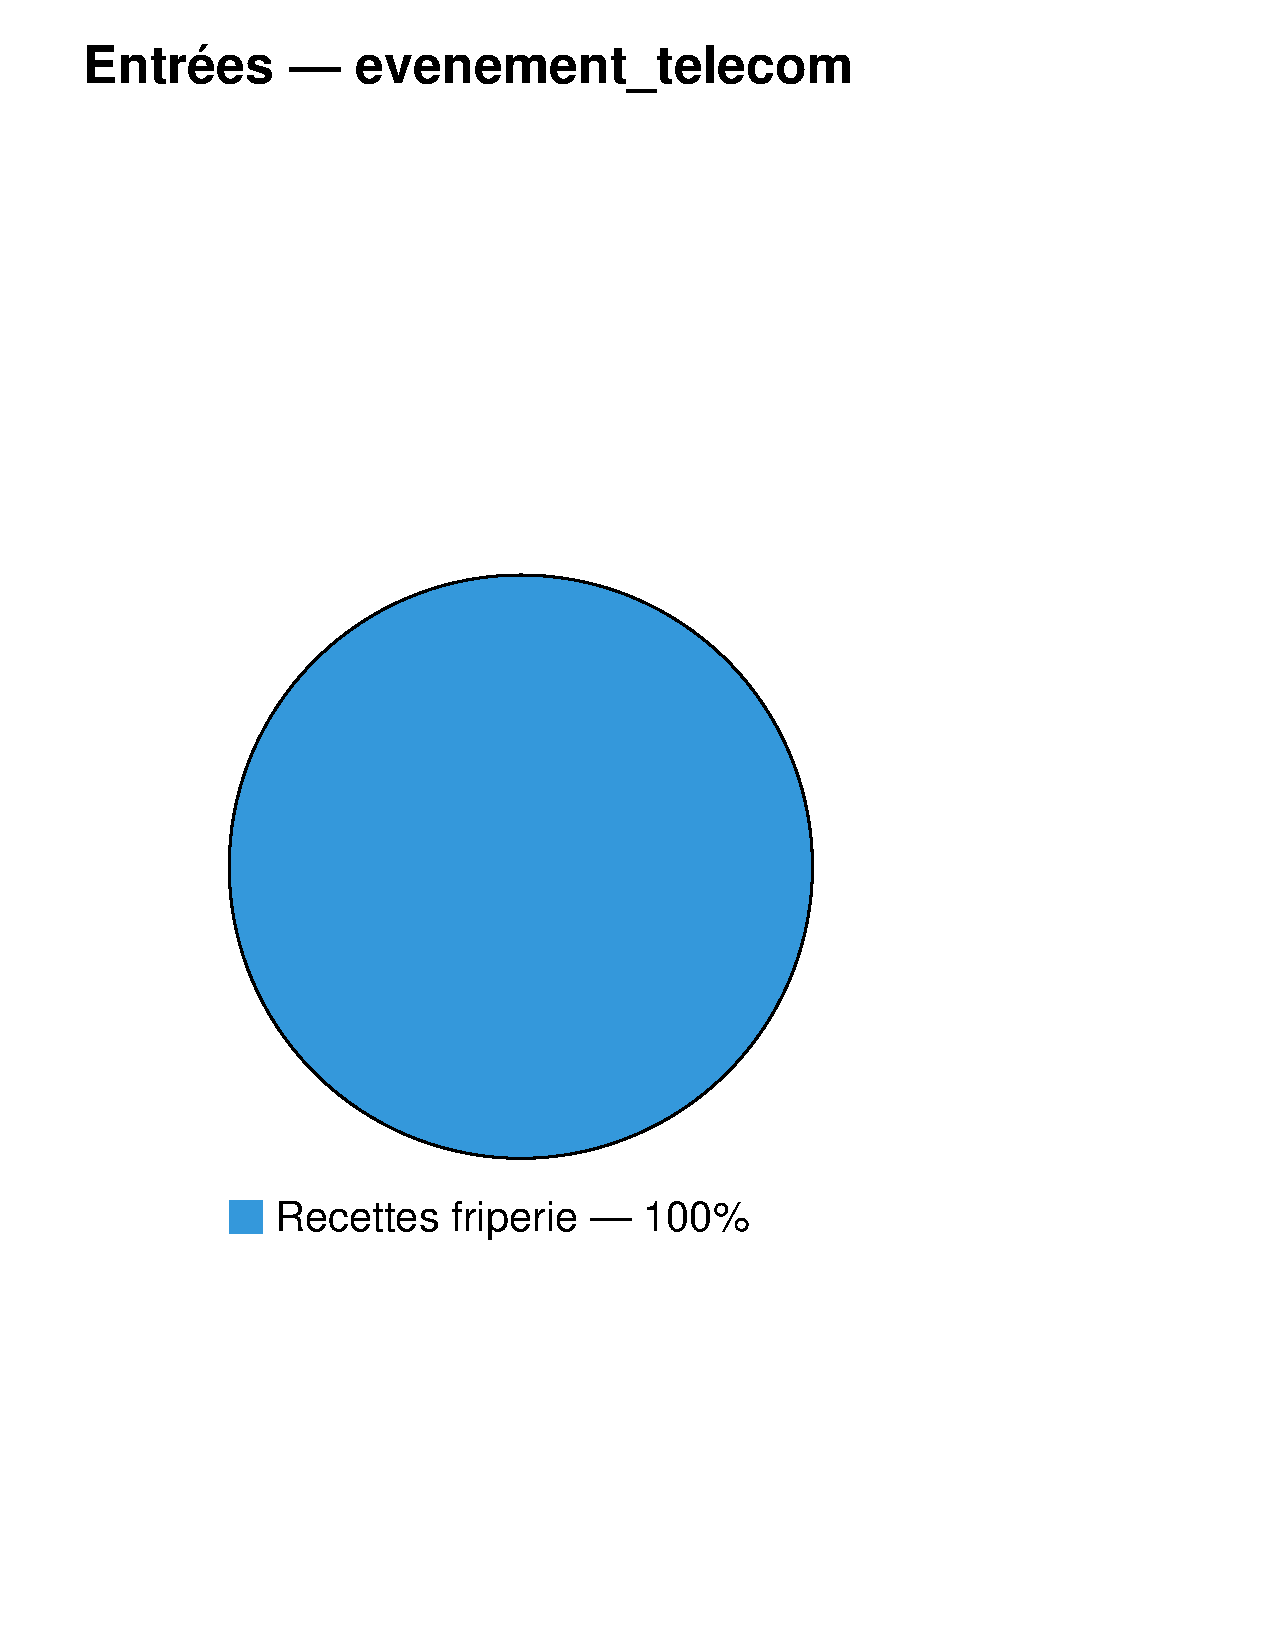
\includegraphics[width=0.46\textwidth]{charts/evenement_telecom_income.pdf}
\hfill

\includegraphics[width=0.46\textwidth]{charts/evenement_telecom_expense.pdf}
\end{center}

\bigskip
\textbf{Bilan activité :} \EUR{147.00}

\newpage
\section*{evenement\_telespoir}

\subsection*{Tableau des écritures}
\rowcolors{2}{softgray}{white}
\begin{longtable}{L{2.7cm} L{8.2cm} R{3.0cm}}
\toprule
\textbf{Date} & \textbf{Description} & \textbf{Montant} \\
\midrule
 & Subvention IPP Tompotla & \EUR{4275.00} \\
01/06/2023 & lot TomPOTla & \EUR{-136.00} \\
01/06/2023 & Lot enceinte tompotla & \EUR{-34.99} \\
02/06/2023 & Lot TomPOTla & \EUR{-170.99} \\
07/06/2023 & Recettes KFT x Télespoir & \EUR{100.00} \\
09/02/2024 & Bières TomPotla & \EUR{-490.00} \\
10/03/2023 & Préstation Soirée TomPOTla & \EUR{-375.00} \\
12/02/2024 & Présatation Boissons BDE & \EUR{-431.70} \\
15/01/2024 & places et tickets & \EUR{41.42} \\
15/04/2023 & lot TomPOTla & \EUR{-339.99} \\
15/04/2023 & lot TomPOTla & \EUR{-118.00} \\
15/04/2023 & lot TomPOTla & \EUR{-150.00} \\
15/05/2023 & TomPOTla & \EUR{-320.90} \\
16/01/2024 & places et tickets & \EUR{8.67} \\
16/01/2024 & places et tickets & \EUR{59.74} \\
18/01/2024 & places et tickets & \EUR{11.61} \\
19/01/2024 & places et tickets & \EUR{192.66} \\
19/04/2023 & stand Ekiden & \EUR{-232.22} \\
19/04/2023 & stand Ekiden & \EUR{-193.41} \\
20/01/2024 & Photo TomPotla & \EUR{-100.00} \\
20/04/2023 & Stand bouffe ekiden & \EUR{152.91} \\
20/06/2023 & Sécurité TomPOTla & \EUR{-1150.85} \\
21/06/2023 & Prestation repas staffeurs & \EUR{820.00} \\
22/01/2024 & places et tickets & \EUR{245.81} \\
22/06/2023 & Recettes Télébreizh & \EUR{102.47} \\
23/01/2024 & places et tickets & \EUR{581.01} \\
23/01/2024 & places et tickets & \EUR{1.83} \\
24/10/2023 & Bingo 2024 & \EUR{22.98} \\
24/10/2023 & Bingo & \EUR{29.21} \\
24/10/2023 & Bingo & \EUR{48.40} \\
25/10/2023 & Bingo & \EUR{163.89} \\
26/02/2024 & Sécurité TomPOTla & \EUR{-503.50} \\
26/04/2023 & Prestation soirée TompPotla & \EUR{-150.00} \\
26/10/2023 & Bingo & \EUR{434.72} \\
27/02/2024 & lot TomPOTla & \EUR{-239.10} \\
27/10/2023 & Bingo & \EUR{32.25} \\
28/02/2024 & Prestation soirée TompPotla & \EUR{-150.00} \\
29/02/2024 & lot TomPOTla & \EUR{-741.70} \\
30/06/2023 & Recettes Télébreizh & \EUR{204.34} \\
30/06/2023 & Recettes Télébreizh & \EUR{20.81} \\

\bottomrule
\end{longtable}
\rowcolors{2}{}{}

\subsection*{Répartition}
\begin{center}
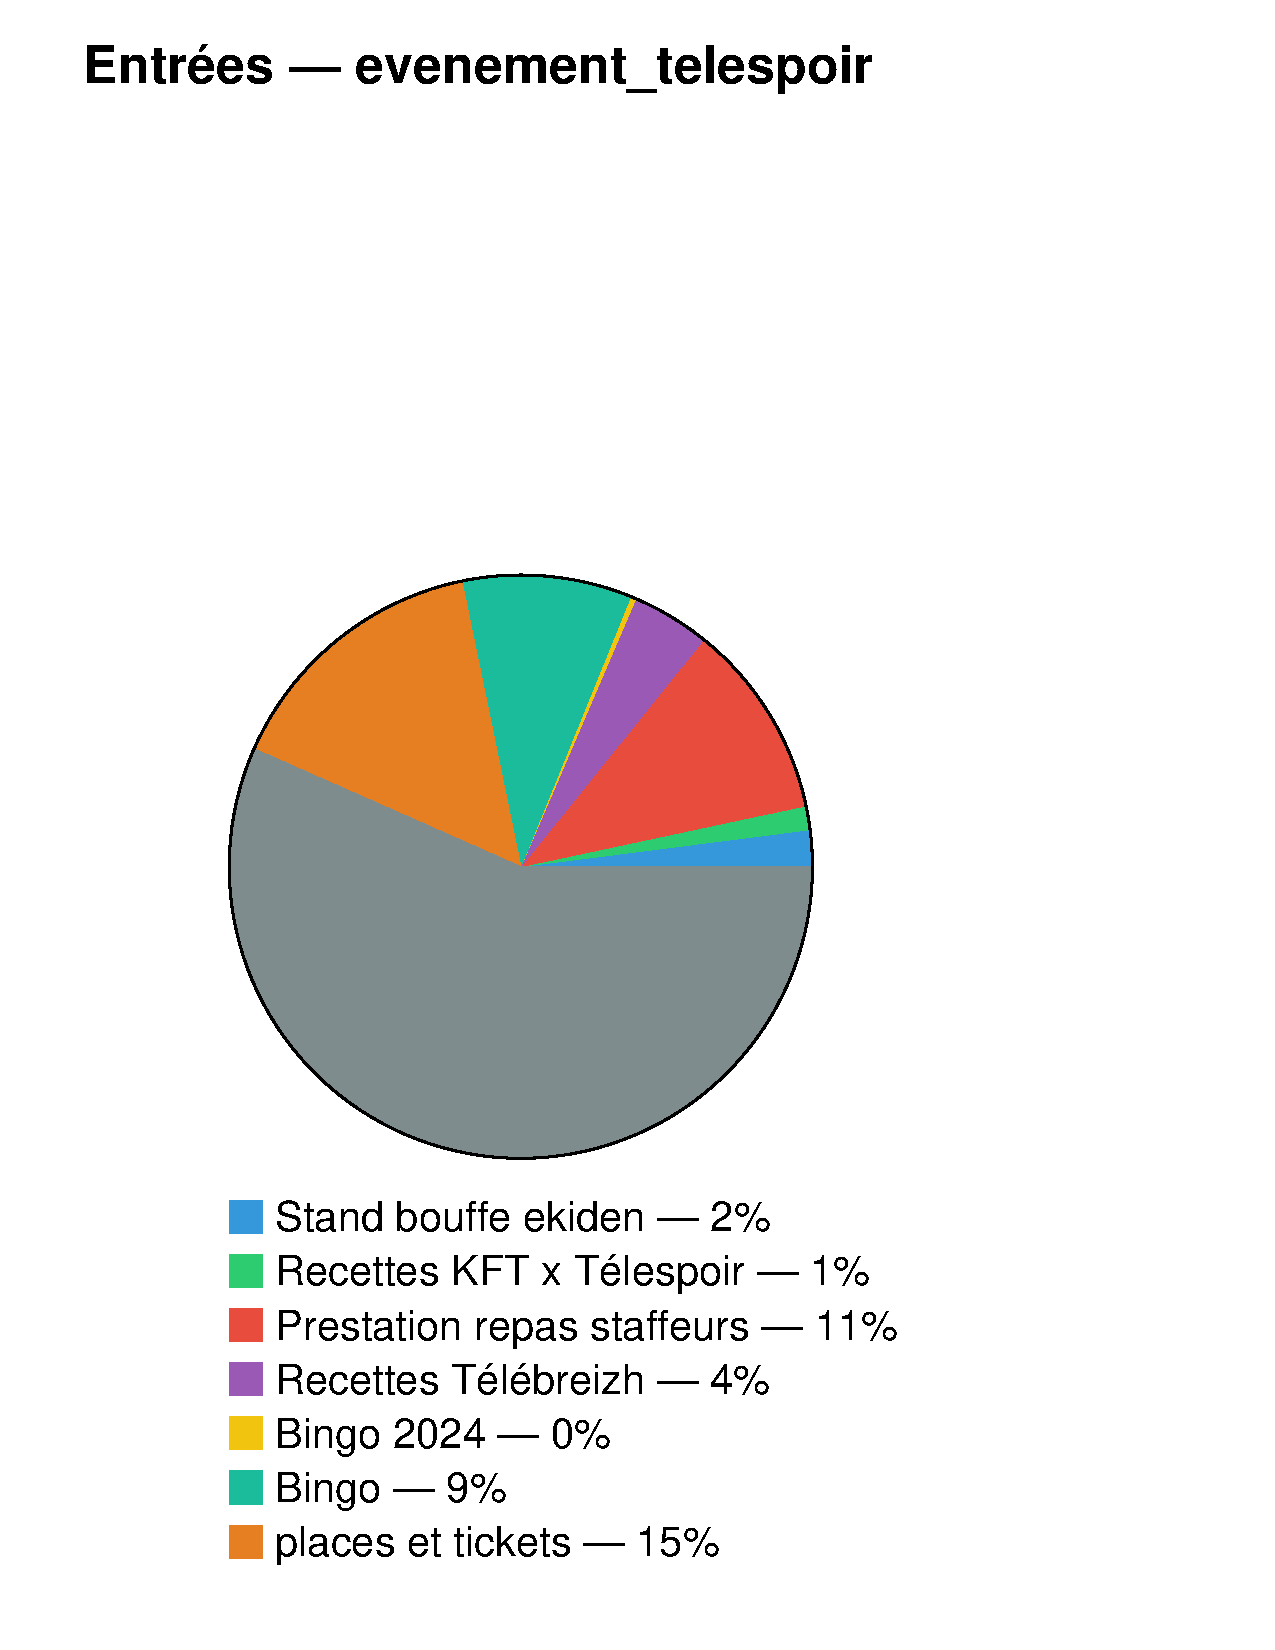
\includegraphics[width=0.46\textwidth]{charts/evenement_telespoir_income.pdf}
\hfill
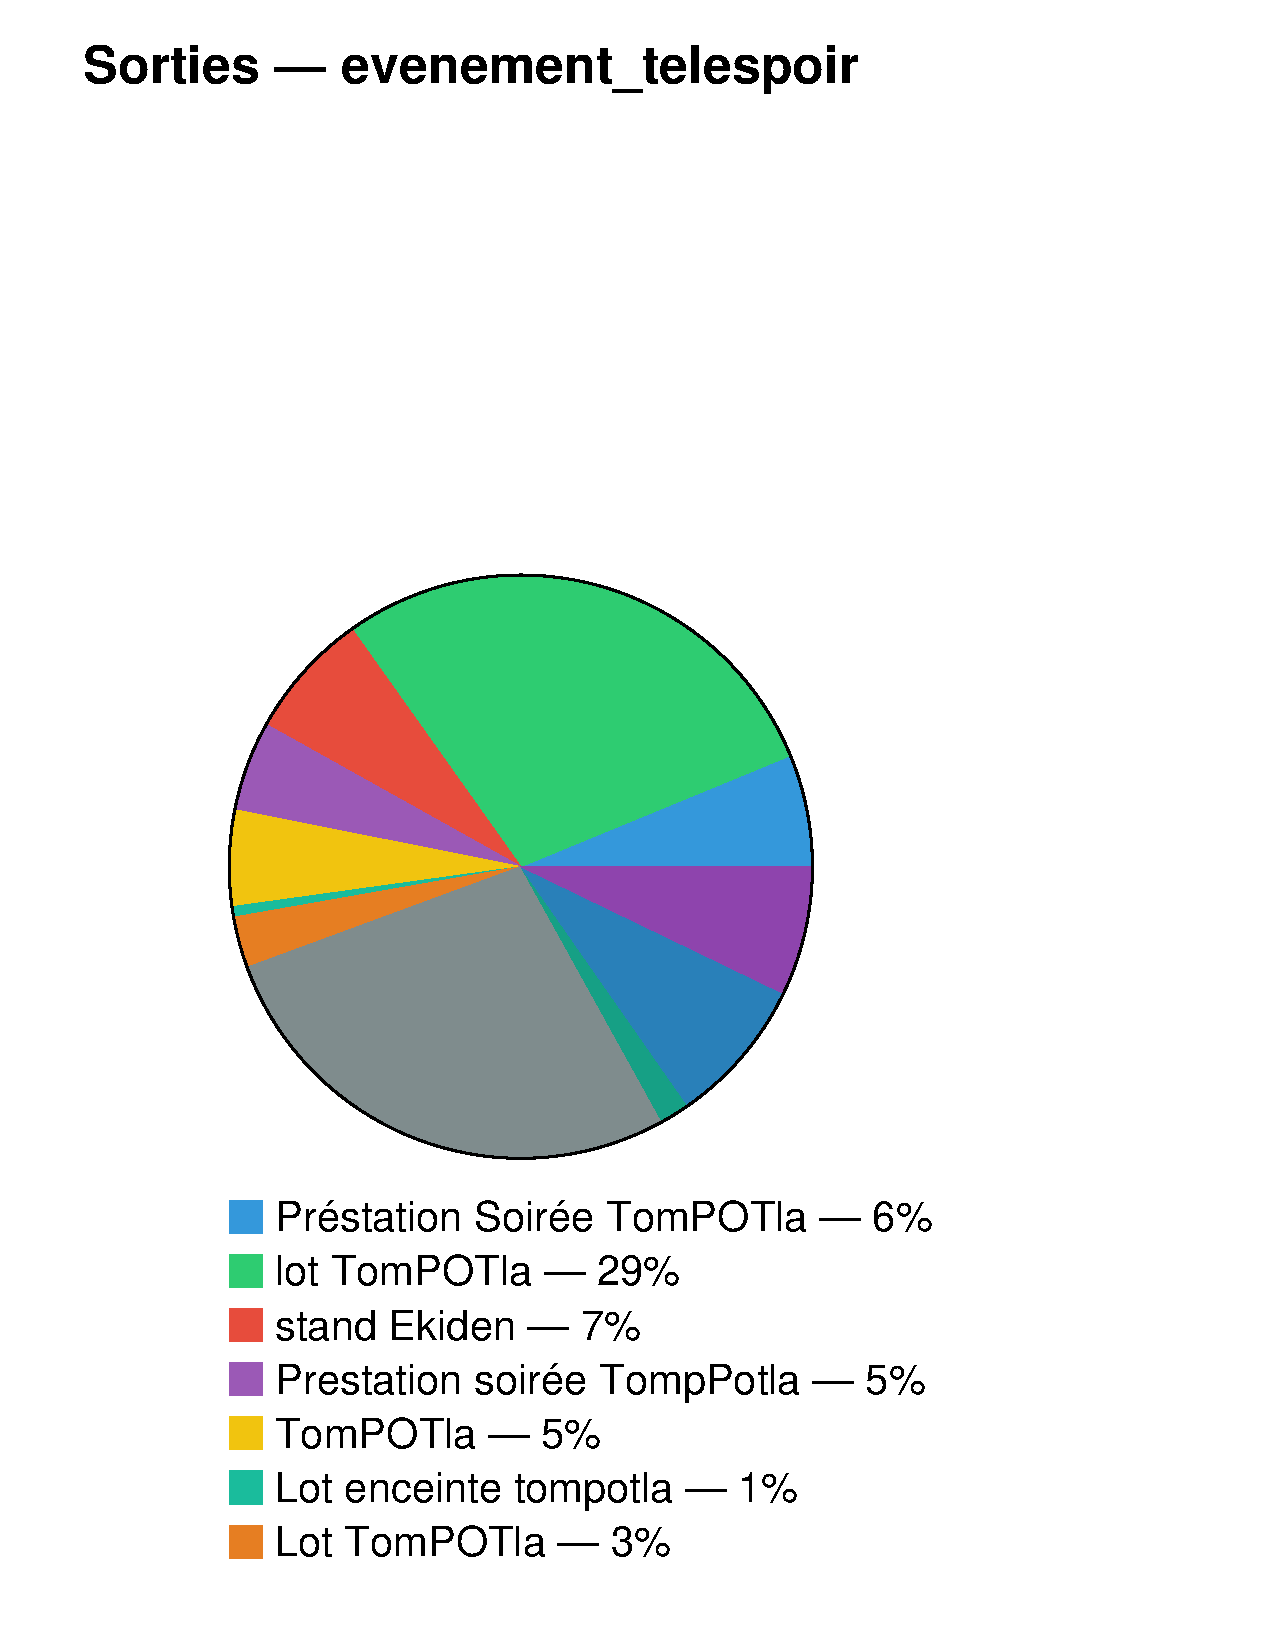
\includegraphics[width=0.46\textwidth]{charts/evenement_telespoir_expense.pdf}
\end{center}

\bigskip
\textbf{Bilan activité :} \EUR{1521.38}

\newpage
\section*{maraude}

\subsection*{Tableau des écritures}
\rowcolors{2}{softgray}{white}
\begin{longtable}{L{2.7cm} L{8.2cm} R{3.0cm}}
\toprule
\textbf{Date} & \textbf{Description} & \textbf{Montant} \\
\midrule
08/06/2023 & maraude 2 & \EUR{-16.90} \\
13/04/2023 & Premières courses Maraude & \EUR{-28.28} \\
13/04/2023 & Premières courses Maraude & \EUR{-27.78} \\
13/04/2023 & Premières courses Maraude & \EUR{-32.36} \\
15/02/2024 & Maraude 4 & \EUR{-79.91} \\
24/10/2023 & maraude 3 & \EUR{-48.33} \\
24/10/2023 & maraude 3 & \EUR{-43.26} \\

\bottomrule
\end{longtable}
\rowcolors{2}{}{}

\subsection*{Répartition}
\begin{center}

\includegraphics[width=0.46\textwidth]{charts/maraude_income.pdf}
\hfill
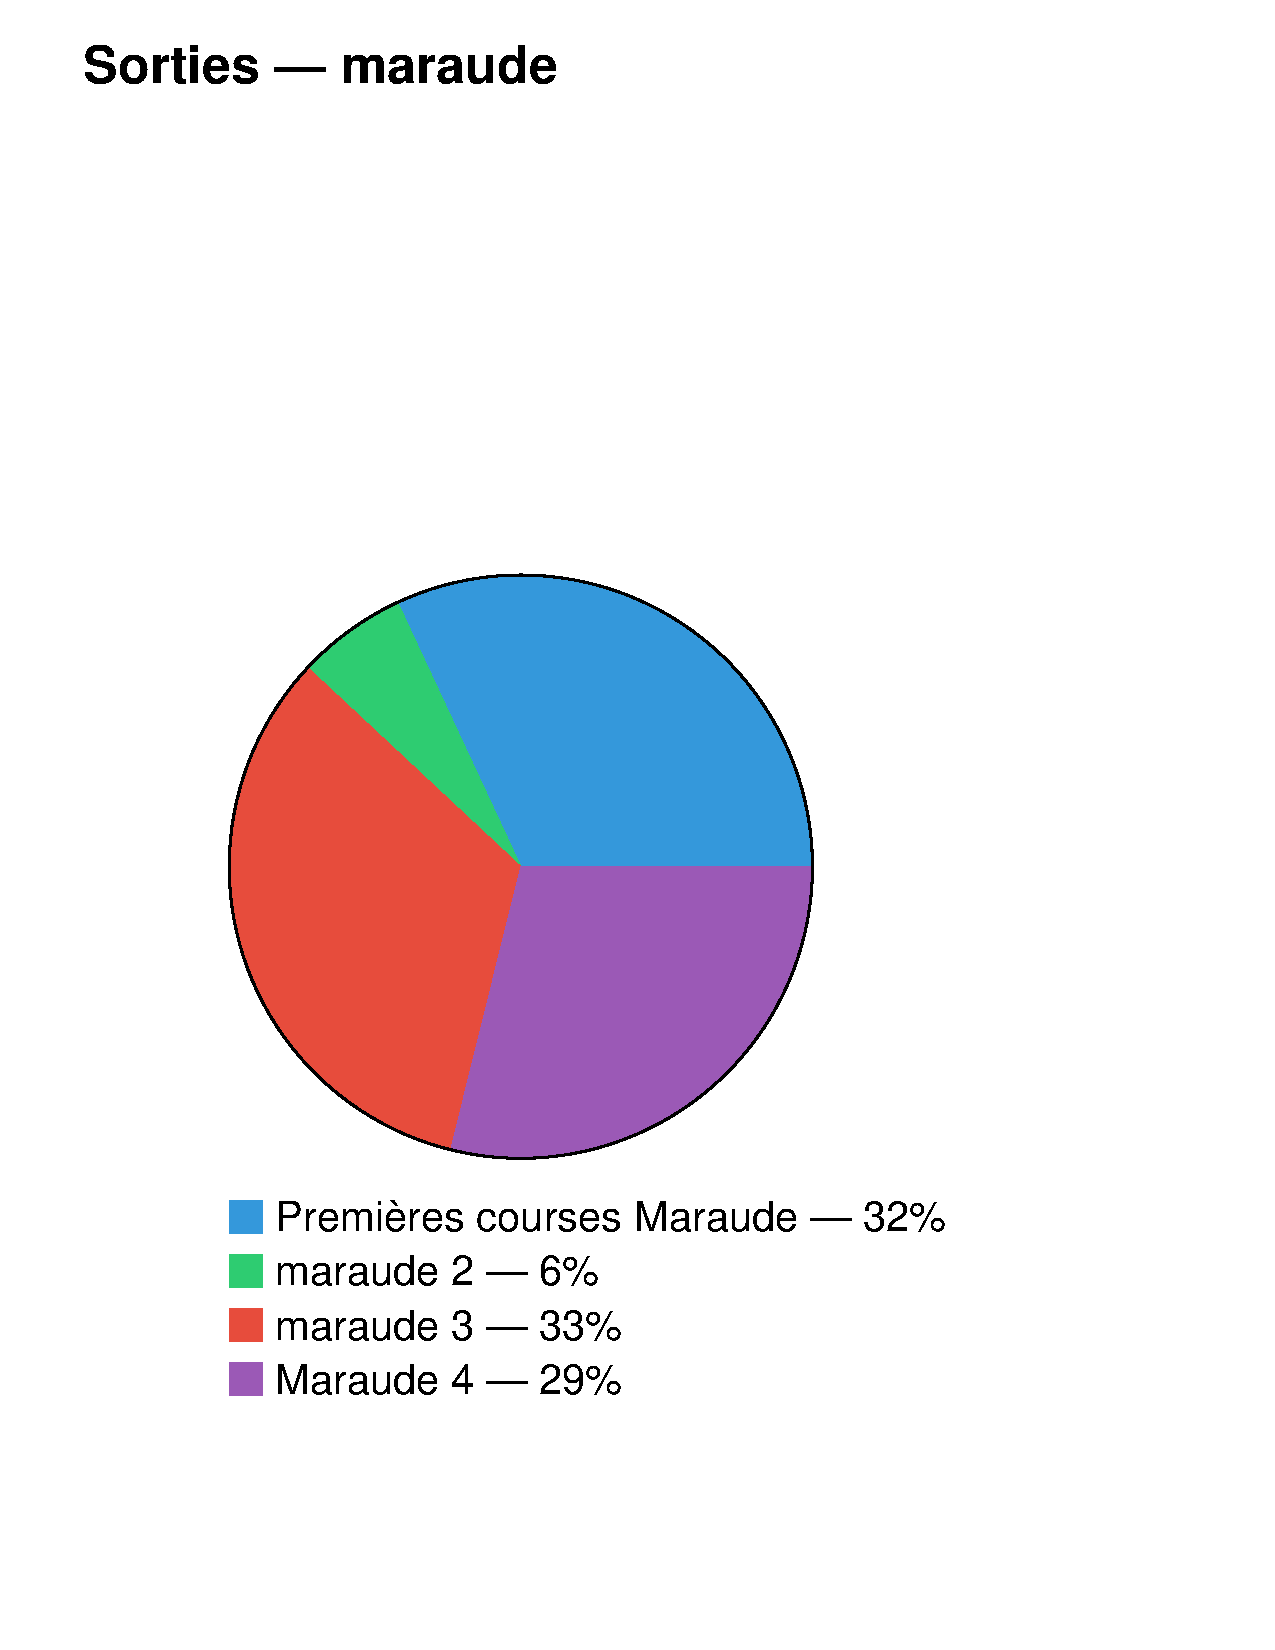
\includegraphics[width=0.46\textwidth]{charts/maraude_expense.pdf}
\end{center}

\bigskip
\textbf{Bilan activité :} \EUR{-276.82}

\newpage
\section*{mission\_humanitaire}

\subsection*{Tableau des écritures}
\rowcolors{2}{softgray}{white}
\begin{longtable}{L{2.7cm} L{8.2cm} R{3.0cm}}
\toprule
\textbf{Date} & \textbf{Description} & \textbf{Montant} \\
\midrule
01/07/2023 & Total Mission & \EUR{-9314.26} \\
03/07/2023 & Don billets et autres & \EUR{1222.15} \\
04/07/2023 & Don billets et autres & \EUR{733.00} \\
07/06/2023 & Don billet Célio & \EUR{732.15} \\
27/06/2023 & Don billet Hamza & \EUR{764.55} \\
27/06/2023 & Don billets et autres & \EUR{2885.30} \\

\bottomrule
\end{longtable}
\rowcolors{2}{}{}

\subsection*{Répartition}
\begin{center}
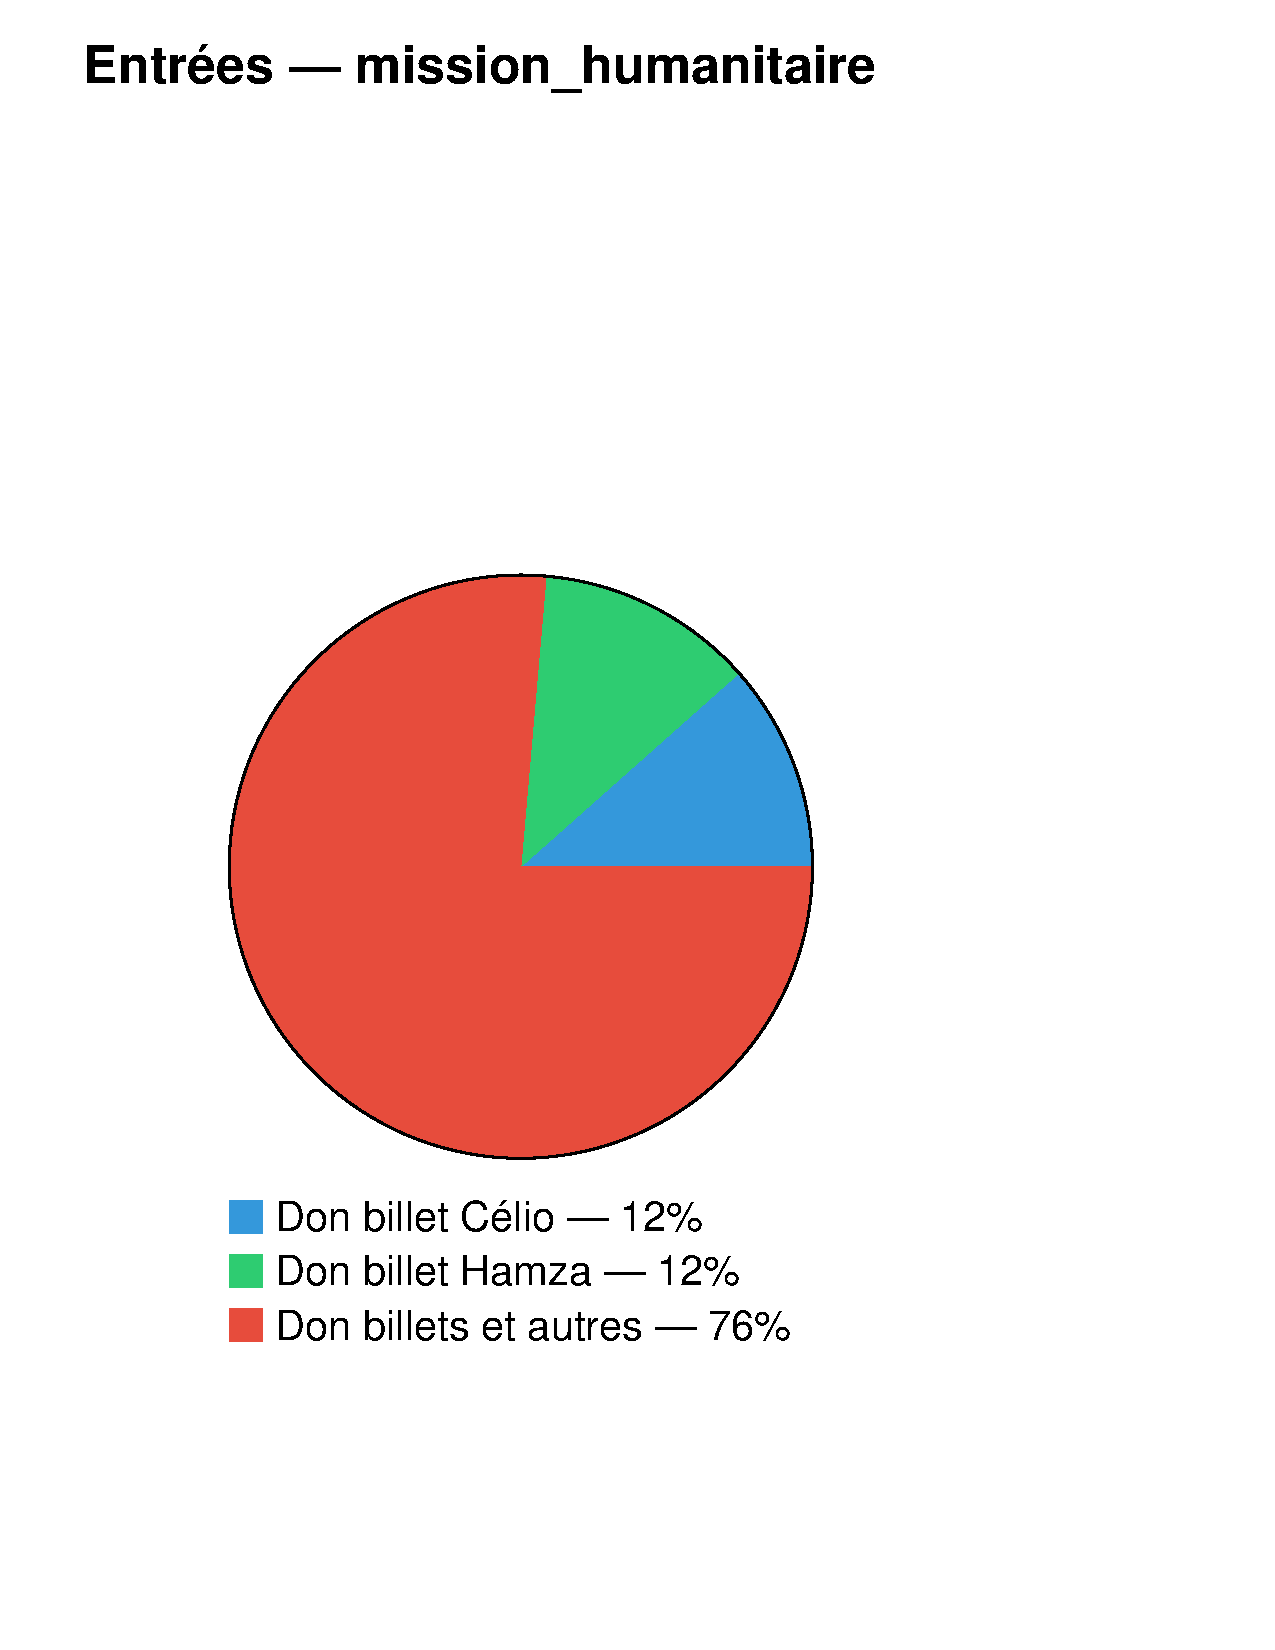
\includegraphics[width=0.46\textwidth]{charts/mission_humanitaire_income.pdf}
\hfill
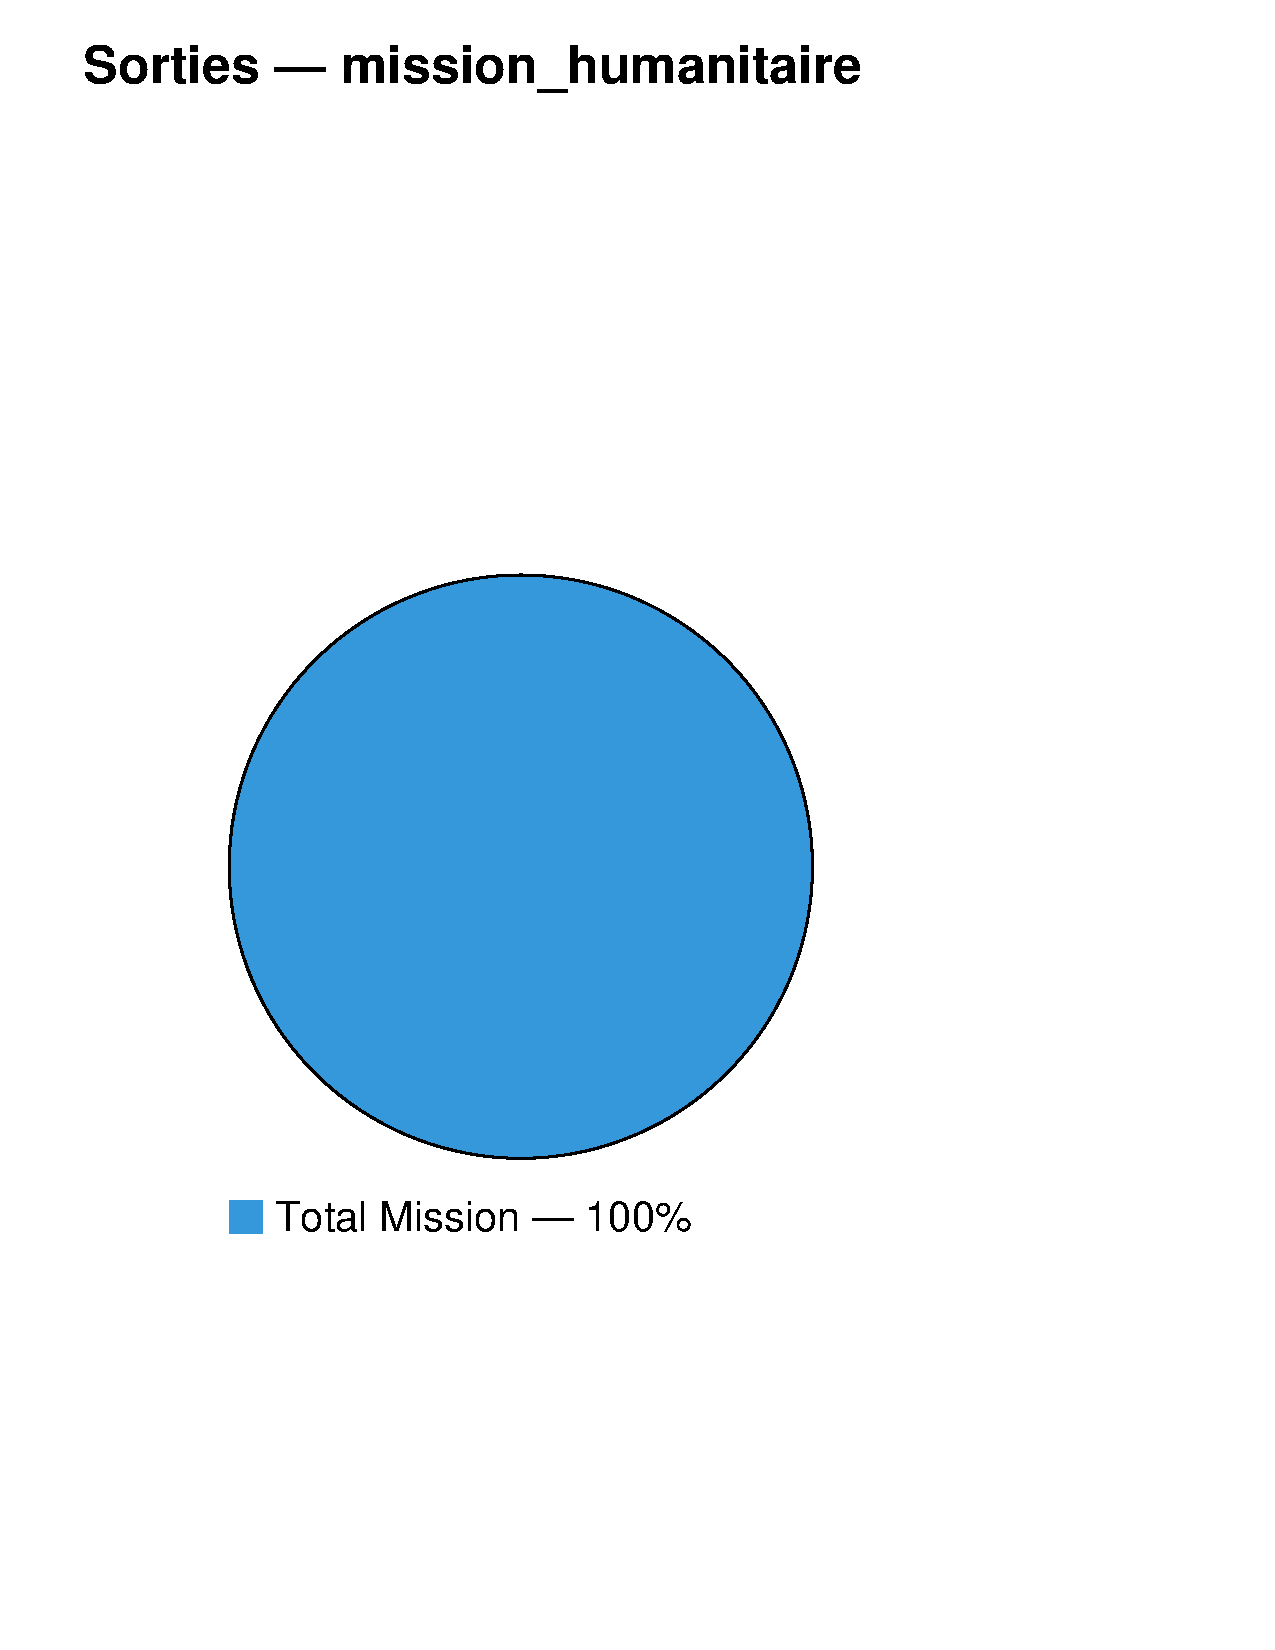
\includegraphics[width=0.46\textwidth]{charts/mission_humanitaire_expense.pdf}
\end{center}

\bigskip
\textbf{Bilan activité :} \EUR{-2977.11}

\newpage


\section*{Bilan final}
\begin{itemize}
  \item Total entrées : \EUR{20483.88}
  \item Total sorties : \EUR{16949.47}
  \item \textbf{Bilan net : \EUR{3534.41}}
\end{itemize}

\end{document}
